\documentclass[12pt,fleqn]{article}\usepackage{../../common}
\begin{document}
Balonlar Ne Zaman Patlar?

Ekonomik krizlerin finans bağlamında kriz öncesi piyasalarda balon
oluşturduğu iddia edilir; mesela ABD'nin 1929, 1987 krizleri, borsalardaki
aşırı çıkışlar ardından düşüş ile başlamıştır, en son 2008 krizi öncesi
emlak piyasasında balon oluşmuştur. Aynı dinamik tek bir sektör endeksi, ya
da tek senet bazında da görülebilmektedir. Demek ki bu tür dinamiği
anlayabilmek, tanıyabilmek, hatta nihai gidişatını tahmin edebilmek
yatırımcı için değerli bir yetenek olabilir.

Bu alanda Didier Sornette'in araştırmaları var [1,2], ona göre balonlar
fiyat zaman serisindeki artışın üstel artışı (exponential increase) bile
geçip süper üstel artış haline gelmesi durumudur. Bu gidişat borsacıların,
finansçılar, finans merkezlerinin birbiri ile çok yönlü etkileşimi
sonucunda oluşur, ve nihai bir patlama noktası vardır. Sornette modeline
deprem tahmin etme amacı ile başlamıştır, ardından aynı yaklaşımı finans
balonlarına da uygulayabileceğini farketmiştir. 

Model alttaki formüldür:

$$ \ln(p(t)) = A + B(t_c - t)^\beta 
\big[ 1 + C \cos (\omega \ln(t_c-t) + \phi )  \big] 
\mlabel{1}
$$

Türetilmesiyle ilgili detaylar ve referanslar yazının sonunda bulunabilir.

Formülü kullanmak için onu bilinen krizlerden önce elde olan veriye
uyduracağız. Normal şartlarda yapılacak budur, bir varlığın, endeksin
gidişatının balon olup olmadığı, eğer balon ise ne zaman patlayabileceği
merak konusudur. Örnek olarak 1929 ve 1987 krizlerini seçtik. 

Ekim 1929 krizi Amerika'da ``Büyük Depresyon'' adı verilen dönemin
başlangıcıydı, ve kriz öncesi Dow Jones (DJIA) endeksinde müthiş bir artış
ardından düşüş gerçekleşti.

\begin{minted}[fontsize=\footnotesize]{python}
import statsmodels.tsa.stattools as st
import pandas as pd, zipfile
with zipfile.ZipFile('data.zip', 'r') as z:
    dfj =  pd.read_csv(z.open('djia.csv'),index_col='Date',parse_dates=True)
    dfs =  pd.read_csv(z.open('sp500.csv'),index_col='Date',parse_dates=True)
    dfi =  pd.read_csv(z.open('ibb.csv'),index_col='Date',parse_dates=True)
\end{minted}

\begin{minted}[fontsize=\footnotesize]{python}
dfj['Adj Close'].plot()
plt.plot()
plt.savefig('tser_bubble_01.png')
\end{minted}

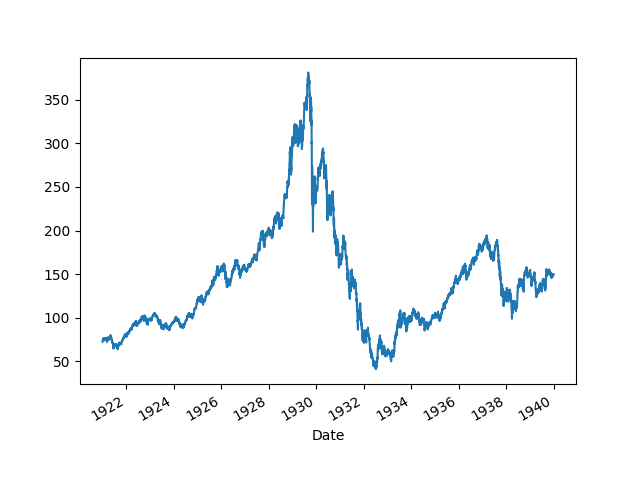
\includegraphics[height=6cm]{tser_bubble_01.png}

Acaba DJIA bu evrede bir balon muydu?  Sornette'in denklemini kriz öncesi
veriye uyduralım,

\begin{minted}[fontsize=\footnotesize]{python}
import pandas as pd
from lmfit import Parameters, minimize
from lmfit.printfuncs import report_fit

def init_fit(min, max, init):
    fit_params = Parameters()
    fit_params.add('tc', value=init, max=max, min=min)
    fit_params.add('A', value=2.0, max=10.0, min=0.1)
    fit_params.add('m', value=0.5, max=1.0, min=0.01)
    fit_params.add('C', value=0.0, max=2.0, min=-2)
    fit_params.add('beta', value=0.5, max=1.0, min=0.1)
    fit_params.add('omega', value=20., max=40.0, min=0.1)
    fit_params.add('phi', value=np.pi, max=2*np.pi, min=0.1)
    return fit_params

def f(pars,x):
    tc = pars['tc'].value
    A = pars['A'].value
    m = pars['m'].value
    C = pars['C'].value
    beta = pars['beta'].value
    omega = pars['omega'].value
    phi = pars['phi'].value
    tmp1 = (1 + C*np.cos(omega*np.log(tc-x) + phi))
    model = A - ((m*((tc-x)**beta))*tmp1)
    return model
    
def residual(pars,y,t):
    return y-f(pars,t)

fit_params = init_fit(1922.0,1940.,1939)

dfj = dfj[(dfj.index >= '1922-01-01')&(dfj.index <= '1929-01-01')]
dfj['DecDate'] = np.linspace(1922,1929,len(dfj))

y = np.log(dfj['Adj Close'])
t = dfj['DecDate']
out = minimize(residual, fit_params, args=(y,t,))

report_fit(fit_params)
\end{minted}

\begin{verbatim}
[[Variables]]
    tc:      1930.26611 +/- 0.060428 (0.00%) (init= 1939)
    A:       6.06304875 +/- 0.043302 (0.71%) (init= 2)
    m:       0.46154101 +/- 0.027743 (6.01%) (init= 0.5)
    C:       0.07785667 +/- 0.003250 (4.17%) (init= 0)
    beta:    0.62152034 +/- 0.019028 (3.06%) (init= 0.5)
    omega:   10.7292149 +/- 0.176101 (1.64%) (init= 20)
    phi:     6.28318123 +/- 6.869443 (109.33%) (init= 3.141593)
[[Correlations]] (unreported correlations are <  0.100)
    C(omega, phi)                =  0.995 
    C(m, beta)                   = -0.994 
    C(tc, phi)                   =  0.982 
    C(tc, omega)                 =  0.963 
    C(A, m)                      =  0.960 
    C(A, beta)                   = -0.925 
    C(m, C)                      = -0.918 
    C(A, C)                      = -0.917 
    C(C, beta)                   =  0.903 
    C(tc, A)                     =  0.759 
    C(A, phi)                    =  0.726 
    C(A, omega)                  =  0.697 
    C(tc, C)                     = -0.623 
    C(C, phi)                    = -0.589 
    C(C, omega)                  = -0.559 
    C(tc, m)                     =  0.553 
    C(m, phi)                    =  0.518 
    C(m, omega)                  =  0.489 
    C(tc, beta)                  = -0.470 
    C(beta, phi)                 = -0.434 
    C(beta, omega)               = -0.404 
\end{verbatim}

Formül yılı ondalık yıl (decimal date) formatında istiyor, bu sebeple bazı
ek işlemler yapıldı.

Uyumdan gelen sonuç balon patlama anı $t_c$ olarak 1930 başını verdi. Ve
kriz 1929 sonunda gerçekleşti. İyi bir hesap. Dikkat, hesap için 1929
yılının verisini bile almadık ve 1929 sonu 1930 başını elde ettik. Acaba
uyum istatiksel olarak ne kadar iyi?  Cevap için uyumdan gelen artıklara
bakabiliriz, normal regresyonda artıkların gürültü, yani Gaussian dağılıma
sahip olmasını kontrol ediyorduk, zaman serisi uyumu için artıkların
ortalamaya-dönüşe (mean-reversion) sahip olup olmadığını kontrol
edebiliriz. Bunun için ADF testimiz var,

\begin{minted}[fontsize=\footnotesize]{python}
res = list(st.adfuller(out.residual,maxlag=1))
print res[0], '%1,%5,%10', res[4]['1%'], res[4]['5%'], res[4]['10%']
\end{minted}

\begin{verbatim}
-3.94947024619 %1,%5,%10 -3.43409223882 -2.86319299 -2.56765000294
\end{verbatim}

Test artıkların yüzde 99 ihtimalle ortalamaya dönüşe sahip olduğunu
söylüyor. 

Uydurulan fonksiyonu veriyle beraber gösterelim,

\begin{minted}[fontsize=\footnotesize]{python}
dfj['Sornette'] = np.exp(f(fit_params, dfj.DecDate))
dfj[['Adj Close','Sornette']].plot()
plt.savefig('tser_bubble_04.png')
\end{minted}

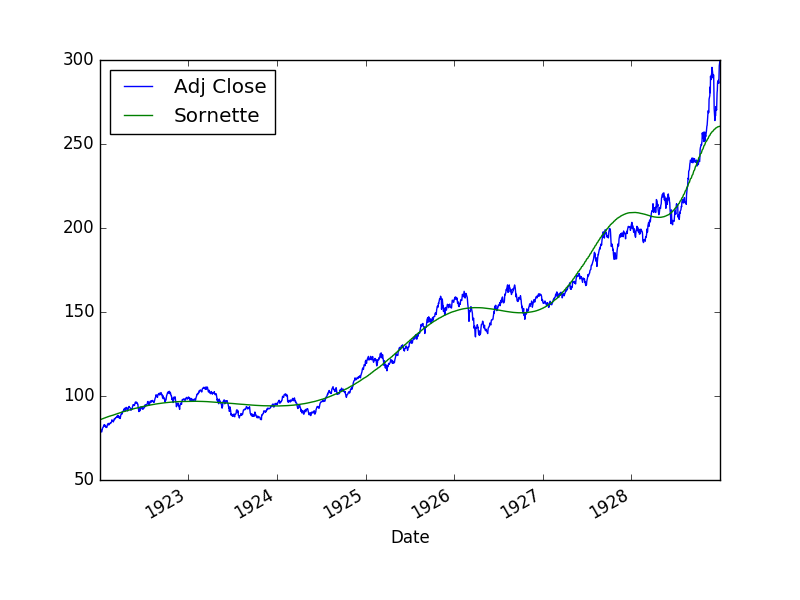
\includegraphics[height=6cm]{tser_bubble_04.png}

Uyum oldukça iyi. Acaba balon patlama sorusunu daha az veriyle sorsaydık ne
olurdu? Yani, acaba, eldeki verinin iki senesini daha silsek, yani aşırı
yükselişin olmadığı zamandaki veriyle bir daha hesap yapsak ne cevap
alırdık? Modele göre aynı cevabı almamamız gerekir, çünkü formül aşırı
çıkışları yakalıyor, ve DJIA'in kriz öncesi son anlarında aşırı çıkış
vardı.

\begin{minted}[fontsize=\footnotesize]{python}
fit_params2 = init_fit(1922.0,1940.,1939.)
dfj2 = dfj[:-600] # son iki sene verisini attik
y2 = np.log(dfj2['Adj Close'])
t2 = dfj2['DecDate']
out2 = minimize(residual, fit_params2, args=(y2,t2,))
res2 = list(st.adfuller(out2.residual,maxlag=1))
print res2[0], '%1,%5,%10', res[4]['1%'], res[4]['5%'], res[4]['10%']
\end{minted}

\begin{verbatim}
-2.01491805971 %1,%5,%10 -3.43409223882 -2.86319299 -2.56765000294
\end{verbatim}

\begin{minted}[fontsize=\footnotesize]{python}
print fit_params2['tc'].value 
\end{minted}

\begin{verbatim}
1926.91504363
\end{verbatim}

Testler yüzde 90 aralığına bile yaklaşamadı. Uyum başarılı değil.

Kara Pazartesi (Black Monday)

Ekim 19, 1987'da S\&P 500 büyük bir düşüş yaşadı ve bu gün tarihe Kara
Pazartesi olarak geçti. Büyük düşüş öncesi oluşan çıkışın balon olduğu
iddia edilmektedir.

\begin{minted}[fontsize=\footnotesize]{python}
dfs['Adj Close'].plot()
plt.savefig('tser_bubble_02.png')
\end{minted}

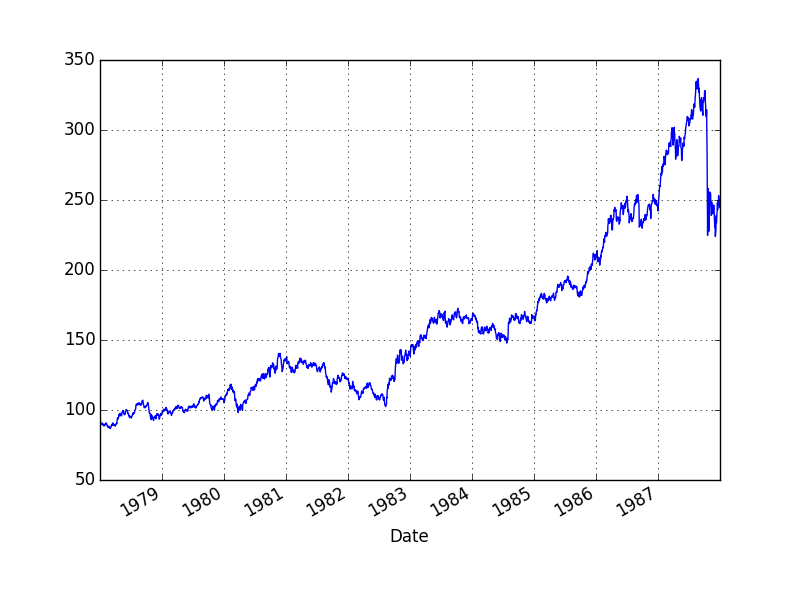
\includegraphics[height=6cm]{tser_bubble_02.png}

\begin{minted}[fontsize=\footnotesize]{python}
dfs = dfs[(dfs.index < '1987-10-18')] # kara ptesi oncesini al
beg_date = dfs.head(1).index[0].timetuple()
beg_date_dec = beg_date.tm_year + (beg_date.tm_yday / 367.)
end_date = dfs.tail(1).index[0].timetuple()
end_date_dec = end_date.tm_year + (end_date.tm_yday / 367.)
dfs['DecDate'] = np.linspace(beg_date_dec,end_date_dec,len(dfs))

fit_params3 = init_fit(1970.,1995.,1989.)
y3 = np.log(dfs['Adj Close'])
t3 = dfs['DecDate']
out3 = minimize(residual, fit_params3, args=(y3,t3,))
report_fit(fit_params3)
\end{minted}

\begin{verbatim}
[[Variables]]
    tc:      1987.78746 +/- 0.001713 (0.00%) (init= 1989)
    A:       2.16393842 +/- 0.780555 (36.07%) (init= 2)
    m:       0.44165592 +/- 0.757581 (171.53%) (init= 0.5)
    C:       0.00092504 +/- 0.121291 (13112.07%) (init= 0)
    beta:    0.45100463 +/- 0.517380 (114.72%) (init= 0.5)
    omega:   20.2695125 +/- 239.2351 (1180.27%) (init= 20)
    phi:     2.80991123 +/- 440.6670 (15682.60%) (init= 3.141593)
[[Correlations]] (unreported correlations are <  0.100)
    C(m, beta)                   = -0.988 
    C(A, m)                      =  0.986 
    C(omega, phi)                = -0.958 
    C(A, beta)                   = -0.951 
    C(tc, A)                     =  0.209 
    C(tc, m)                     =  0.206 
    C(tc, beta)                  = -0.198 
    C(C, beta)                   =  0.117 
\end{verbatim}

Cevap kabaca Kara Pazartesi anını yakaladı! Artıkları kontrol edelim,

\begin{minted}[fontsize=\footnotesize]{python}
res3 = list(st.adfuller(out3.residual,maxlag=1))
print res3[0], '%1,%5,%10', res[4]['1%'], res[4]['5%'], res[4]['10%']
\end{minted}

\begin{verbatim}
-2.31790207914 %1,%5,%10 -3.43409223882 -2.86319299 -2.56765000294
\end{verbatim}

Tam yüzde 90-95 aralığına düşmedi, fakat çok uzak ta değil. Bu uyumun fena
olduğu söylenemez.

Biyoteknoloji

Daha yakın zamandan bir örnek verelim. ABD biyoteknoloji hisselerinde
abartılı bir artış olduğu uzun zamandır söylenmekteydi. Biyoteknoloji
sektörünü temsil eden bir ETF olan IBB'nin grafiği alttadır.

\begin{minted}[fontsize=\footnotesize]{python}
dfi['Adj Close'].plot()
plt.savefig('tser_bubble_03.png')
\end{minted}

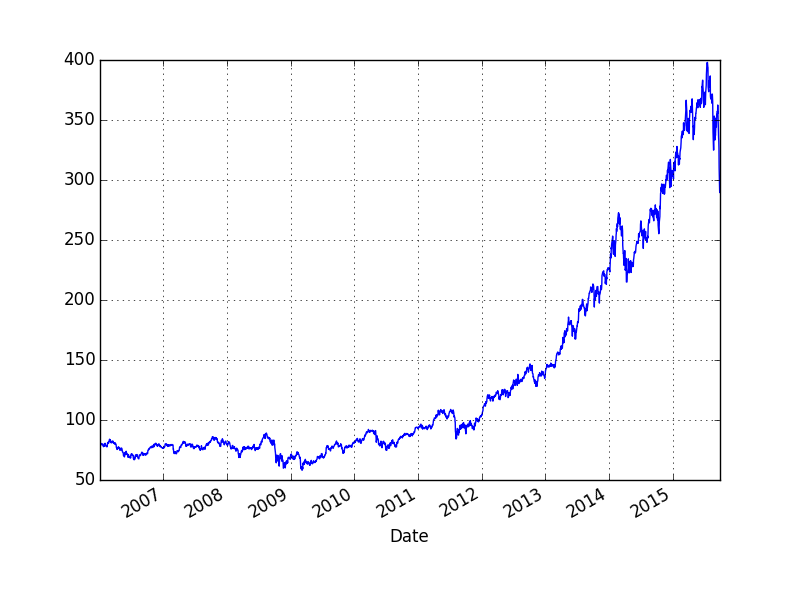
\includegraphics[height=6cm]{tser_bubble_03.png}

Biyoteknoloji balonu 2015'in ikinci bölümünde patladı ve sert bir düşüş
yaşandı. Acaba tekniğimiz bu düşüşü yakalayabilecek mi?

\begin{minted}[fontsize=\footnotesize]{python}
dfi = dfi[(dfi.index < '2015-07-01')] 
beg_date = dfi.head(1).index[0].timetuple()
beg_date_dec = beg_date.tm_year + (beg_date.tm_yday / 367.)
end_date = dfi.tail(1).index[0].timetuple()
end_date_dec = end_date.tm_year + (end_date.tm_yday / 367.)
dfi['DecDate'] = np.linspace(beg_date_dec,end_date_dec,len(dfi))

fit_params4 = init_fit(2012.,2018.,2017.)
y4 = np.log(dfi['Adj Close'])
t4 = dfi['DecDate']
out4 = minimize(residual, fit_params4, args=(y4,t4,))
print fit_params4['tc'].value 
\end{minted}

\begin{verbatim}
2015.51052262
\end{verbatim}

Sonuç olarak 2015 ortası verildi. Uyum nasıl?

\begin{minted}[fontsize=\footnotesize]{python}
res4 = list(st.adfuller(out4.residual,maxlag=1))
print res4[0], '%1,%5,%10', res[4]['1%'], res[4]['5%'], res[4]['10%']
\end{minted}

\begin{verbatim}
-2.34444994145 %1,%5,%10 -3.43409223882 -2.86319299 -2.56765000294
\end{verbatim}

Test sonucu 90-95 aralığına yakın, uyum fena değil. 

Bu teknik borsada alım/satım stratejisi bağlamında otomize olarak
kullanılabilir, ya da belli bazı hisselerden ne zaman uzak durulacağı
konusunda bir alarm vermek için faydalı olabilir.

Türetmek

Sornette'in modelinin başlangıcı bir zaman serisindeki artışının üstel
(exponential) hızı geçtiği zaman sonlu-anda (finite-time) bir eşsizlik
(singularity) çıktığı iddiası [1,4]. Eşsizlik konusunu {\em Diferansiyel
  Denklemler} notlarında işledik; eşsiz nokta bir fonksiyonun analitikliği
kaybettiği yerdir. Peki modelde eşsizliğin ortaya çıkması gerçek hayatta
illa bunun olacağı anlamına geliyor mu? İlginç bir şekilde eğer
matematiksel model sağlam ise eşsizliğin tahmin edildiği yerde hakikaten bu
durum ortaya çıkıyor, mesela izafiyet kuramının matematiği eşsiz noktaların
varlığını tahmin eder, ve hakikaten de tahmin edildiği şekilde uzayda bu
noktalarda kara deliklerin olduğu ispatlanmıştır. Aynı şekilde bir
materyelin kırılması / parçalanması matematiksel modelin eşsizlik
noktasında olur, ve deneylerde bu anda materyel kırılması gözlenmiştir.

Sornette'e göre nüfus artışı, bir ekonominin ürettiği değeri temsil eden
gayrısafi yurtiçi hasıla (gross domestic product -GDP-) artışı rakamlarına
dünya bazında bakarsak üstel üstü artışları görebiliyoruz, ve aynen
materyel kırılmasında olduğu gibi modelin eşsizlik tahmin ettiği yeri ``bir
fazın bittiği an'' olarak görürsek, bu nokta bir tür sürdüremezliğin
geldiği an olacaktır, ve tabiri caizse ``inceldiği yerden kopma''
noktasıdır, ve bunun ötesinde mesela ne daha fazla nüfus artışı, ne de
ekonomik büyüme mümkün değildir. En azından mevcut çevre, mevcut ölçümler
üzerinden ekonomik büyüme dediğimiz şey olmayacaktır. 

Sonlu an eşsizliğine erişmek için mesela normal nüfus artışı modelinden
başlayalım, nüfusu modellemenin en iyi bilinen yolu Lojistik Denklemdir,
bkz [6], [7], [8]. Model şöyledir;

$$ \frac{dp}{dt} = rp(t) [ K - p(t) ] $$

Lojistik modelde bir taşıma kapasitesi $K$ vardır, ve bu kapasitenin daha
fazlasını çevre koşullarının taşıması mümkün değildir. Fakat [4]'teki
referanslara göre şu iddia edilmektedir; $p(t)$ ile birlikte $K$ de
artmaktadır, çünkü araçlarımızı daha iyi kullanıyoruz, sürekli keşifler
yapıyoruz, ilaçlar, gübre çeşitleri, vs. ve yeni bölgelere yayılıyoruz,
yani sürekli taşıma kapasitesini aşıyoruz. Bu durumda, yani $K > p(t)$'in
olduğu durumda lojistik denklemini çözümü patlar, yani uzaklaşır
(divergent) hale gelir ve sonsuza gider. Bu gidiş süresi, eşsizlik öncesi
varışta giden zaman sonludur, yani belli bir büyüklüğü vardır.

Bu durumda denkleme artık hiçbir etkisi olmayan $-p(t)$ denklemden
çıkartılabilir, ve o zaman geri kalanlar $\delta > 1$ olacak şekilde $K
\propto p^{1+\delta}$ kabul edilebilir, yani $K$'nin kendisi $p$'ye oranla 
büyüyor ve arada bir üstel kanun (power law) ilişkisi vardır. Şimdi aynı 
formülü şu şekilde yazarız, 

$$ \frac{dp}{dt} = r [p(t)]^{1+\delta} $$

ki bu formüle göre artış oranı $r [p(t)]^{1+\delta}$ olarak
hızlanmaktadır. Çözelim, 

$$ \int \frac{dp}{p(t)^{1+\delta}} = \int rt$$

$$ \int p(t)^{-1-\delta} \ud p = rt + C $$

$t_c$'ye (ki bir sabit) erişmek amaçlı olarak $C = -rt_c$ tanımlayalım,

$$ \frac{p(t)^{-\delta}}{-\delta} = rt - rt_c $$

$$ p(t)^{-\delta}= -\delta r(t - t_c) $$

$t-t_c = -(t_c-t)$ olduğu için parantez içindeki çıkartma işlemi şu hale
gelir, 

$$ p(t)^{-\delta}= \delta r(t_c - t) $$

İstediğimiz forma yaklaştık çünkü $t_c$'yi eşsizlik anı olarak hesaplamak
istiyoruz, ve $t$ bu andan önceki zamanı temsil ediyor olmalı. Şimdi 
$\alpha = -\frac{1}{\delta}$ tanımlayalım, ve eşitliğin her iki tarafının
$\alpha$ üstünü alalım,

$$ (p(t)^{-\delta})^\alpha= (\delta r )^\alpha (t_c - t)^\alpha $$

Eğer $p(0) = p_0 = (\delta r )^\alpha$ kabul edersek, eşitliğin sol
tarafını basitleştirince,

$$ p(t) = p_0 (t_c - t)^\alpha $$

elde ederiz, ki bu denklemin $t_c$ anında eşsizliği vardır. 

Şimdi bu basit modeli veri üzerinde test edelim. Elimizde bir milyon yıl
geriye giden nüfus modeli var [3], sadece 0'inci yıl ile 1989 arasını alalım,
ve modeli uyduralım ve bilinmeyen parametreleri hesaplamaya uğraşalım. 
Veriyi uydurma amaçlı olarak şu formül daha kullanışlı olabilir,

$$ 
p(t) = A + B(t_c - t)^z 
\mlabel{2} 
$$

\begin{minted}[fontsize=\footnotesize]{python}
import pandas as pd
dfpop = pd.read_csv('wpop.csv',comment='#',sep='\s')
dfpop = dfpop[(dfpop['Year'] >= 0) & (dfpop['Year'] <= 1998)]
\end{minted}

\begin{minted}[fontsize=\footnotesize]{python}
import pandas as pd
import statsmodels.tsa.stattools as st
from lmfit import Parameters, minimize
from lmfit.printfuncs import report_fit

def f(pars,t):
    tc = pars['tc'].value
    z = pars['z'].value
    A = pars['A'].value
    B = pars['B'].value
    model = A + B*((tc - t)**z)
    return model
    
def residual(pars,y,t):
    return y-f(pars,t)
\end{minted}

\begin{minted}[fontsize=\footnotesize]{python}
fit_params = Parameters()
fit_params.add('tc', value=2100.0, min=2000.,max=2400.)
fit_params.add('z', value=-1., min=-5.0,max=5.0)
fit_params.add('A', value=0., min=0.0, max=10.0)
fit_params.add('B', value=20*1000., min=0.0,max=30*1000.0)
y = np.log(np.array(dfpop.Population.astype(float)))
t = np.array(dfpop.Year.astype(float))
out = minimize(residual, fit_params, args=(y,t,))
report_fit(fit_params)
res = list(st.adfuller(out.residual,maxlag=1))
print 'ADF testi', res[0], '%1,%5,%10', res[4]['1%'], res[4]['5%'], res[4]['10%']
\end{minted}

\begin{verbatim}
[[Variables]]
    tc:   2047.37659 +/- 10.86346 (0.53%) (init= 2100)
    z:   -0.24662286 +/- 0.062236 (25.24%) (init=-1)
    A:    2.72771567 +/- 0.669841 (24.56%) (init= 0)
    B:    15.9169748 +/- 2.943371 (18.49%) (init= 20000)
[[Correlations]] (unreported correlations are <  0.100)
    C(z, A)                      = -0.996 
    C(z, B)                      = -0.992 
    C(tc, B)                     =  0.981 
    C(A, B)                      =  0.977 
    C(tc, z)                     = -0.954 
    C(tc, A)                     =  0.926 
ADF testi -3.14127355675 %1,%5,%10 -3.61550910118 -2.94126235749 -2.60919950139
\end{verbatim}

Sonuç +- 10 sene hata payı ile 2047 senesi çıktı. Artıklar üzerinde ADF
testi yaptık, yüzde 95 kesinliğinde artıkların ortalamaya dönüş özelliğine
sahip olduğunu görüyoruz. Model uyumu iyi demek. 

GDP verisine bakalım,

\begin{minted}[fontsize=\footnotesize]{python}
import pandas as pd
dfgdp = pd.read_csv('wgdpreal.csv',comment='#',sep='\s')
dfgdp = dfgdp[(dfgdp['Year'] >= 0) & (dfgdp['Year'] <= 1998)]
\end{minted}

\begin{minted}[fontsize=\footnotesize]{python}
fit_params = Parameters()
fit_params.add('tc', value=2100.0, min=2000.,max=2400.)
fit_params.add('z', value=-1., min=-5.0,max=5.0)
fit_params.add('A', value=0., min=0.0, max=10.0)
fit_params.add('B', value=20*1000., min=0.0,max=30*1000.0)
y = np.log(np.array(dfgdp.GDPPC.astype(float)))
t = np.array(dfgdp.Year.astype(float))
out = minimize(residual, fit_params, args=(y,t,))
report_fit(fit_params)
res = list(st.adfuller(out.residual,maxlag=1))
print 'ADF testi', res[0], '%1-%10', res[4]['1%'], res[4]['5%'], res[4]['10%']
\end{minted}

\begin{verbatim}
[[Variables]]
    tc:   2148.16544 +/- 21.95284 (1.02%) (init= 2100)
    z:   -1.33135253 +/- 0.155306 (11.67%) (init=-1)
    A:    2.81936402 +/- 0.092028 (3.26%) (init= 0)
    B:    6344.88666 +/- 5.51e+03 (86.76%) (init= 20000)
[[Correlations]] (unreported correlations are <  0.100)
    C(z, B)                      = -0.999 
    C(tc, B)                     =  0.987 
    C(tc, z)                     = -0.981 
    C(z, A)                      = -0.928 
    C(A, B)                      =  0.917 
    C(tc, A)                     =  0.861 
ADF testi -2.65894249385 %1-%10 -3.61550910118 -2.94126235749 -2.60919950139
\end{verbatim}

Burada +- 20 sene hata payıyla 2148 çıktı (daha var!), artıklar yine
ortalama dönüşe sahip. Bu demektir ki ekonomik büyüme, mevcut gidişatıyla
patlama yapacaktır ve kritik an bir tür faz sonu (end of a regime) olarak
addedilebilecektir. Mevcut şartlar altında bundan daha fazlası mümkün değil.

Log Salınım (Log Oscillation)

[4,5]'te bu modelin geliştirilerek (1) formülüne nasıl erişildiğinin
detayları bulunabilir. Hikayenin özü şöyle; materyel kırılması ve buna
benzer diğer doğal olaylarda eşsizlik anı öncesi log salınımlar olduğu da
görülmüştür. Bu salınımlara matematiksel olarak erişmek için (2)'deki
formüldeki $z$ üstelinin kompleks sayı olmasına izin verilir, yani $\beta +
i\omega$ formunda olduğu farz edilir, ve bu şekilde türetime devam edince
ortaya (1)'deki log periyodik salınımlar çıkar. Detaylar için
[1,4]. Sornette bu salınım ekinin formülü ``dekore'' ettiğini
söylemektedir, güzel bir kelime seçilmiş, hakikaten bu salınımlar ana
formüle bir ek, onu ``süslüyor'', fakat tabii ki bu sayede eşsizlik
noktasını yakalamamız kolaylaşıyor çünkü uydurma rutinimiz artık verideki
bu salınımları da veride bulmaya uğraşıyor böylece aradığı tüm
parametrelerin kalitesi artmış oluyor.

Sornette bazı kaynaklarda bir değişik türetim şekli daha uyguluyor [1,5];
buna göre $p(t)$ olarak belirttiğimiz $h(t)$, tehlike oranı (hazard rate)
olarak modellenir, ve fiyat serisi $p(t)$ olarak rasgele calculus'tan
gelinerek modelleniyor, ve $h(t)$, $p(t)$'ye sokuluyor, ve ortaya log
salınımlı model çıkıyor. Bu türetişin bazı ilginç bağlantıları var, mesela
tehlike oranının kimi aşırı, kimi az ama hepsi birbiriyle etkileşimde olan
borsacıların birbirini taklit etmesi yüzünden $h(t)$'nin arttığı
modellenmekte, ki bu artış ta bir üstel kanunu takip ediyor. Fizik ve
sosyal modelde birbiri ile aşırı etkileşim sürekli ortaya üstel kanun
çıkartıyor, bunu biliyoruz. Patlama anı ve öncesinde aslında ortada olan
bir kaos değil, kaos {\em yokluğu}. Bütüne bakıldığında biri rasgele bazen
satan, biri rasgele bazen alan borsacıların patlama anı öncesi birdenbire
düzenli bir şekilde hepsi {\em satıyor}. 

Kaynaklar

[1] Sornette, {\em Why Stock Markets Crash}

[2] Sornette, {\em How we can predict the next financial crisis}, \url{https://www.youtube.com/watch?v=C_eFjLZqXt8}

[3] Long, {\em Estimates of World GDP, One Million B.C. - Present}

[4] Sornette, {\em Finite-time singularity in the dynamics of the world population, economic and financial indices}

[5] Geraskin, {\em Everything You Always Wanted to Know about Log Periodic Power Laws for Bubble Modelling but Were Afraid to Ask}

[6] Bayramlı, Diferansiyel Denklemler, {\em Matematiksel Modelleme}

[7] Bayramlı, Gayrı Lineer Dinamik ve Kaos, {\em Ders 1}

[8] Bayramlı, Diferansiyel Denklemler, {\em Ders 5}



\end{document}
